\begin{bibunit}[plainnat]

\chapter{Retrospective Loss: Looking Back to Improve Training of Deep Neural Networks}

Adobe \\

\textbf{Reference:}~\cite{jandial2020retrospective}

\textbf{Keywords:} 

\section{Какую задачу решают авторы?}

\section{Как решают?}

\section{Преимущества подхода}

\section{Мое мнение}

\chapter{Correlation Networks for Extreme Multi-label Text Classification}

\textbf{Reference:}~\cite{xun2020correlation}

\textbf{Keywords:} multi-label text classification, deep learning, label correlation

\textbf{Code:}~\url{https://github.com/XunGuangxu/CorNet}

\section*{Какую задачу решают авторы?}

Задача extreme multi-label text classification (XMTC) состоит в том, чтобы сопоставить тексту набор наиболее релевантных лэйблов.

Пример появления данной задачи на практике: по описанию товара в интернет магазине, найти наиболее подходящие категории, к которым относится товар.

Как и во многих других NLP задачах, Deep Learning подходы дают state-of-the-art результаты. \\

Как правило, XMTC модели состоят из двух компонент: первая - извлекает информацию из текста и строит некоторое представление, вторая - использует полученное представление для предсказания лэйблов.

Существует большое количество разных подходов к построению первой компоненты, но вторая компонента, чаще всего, представляет из себя полносвязный слой (FC). \\

Использование простого FC слоя не позволяет учитывать полезные корреляции между лэйблами. 

Например, если мы уверены в том, что товару соответствуют лэйблы 'Blues' и 'R\&B', то скорее всего также товару должен соотвествовать лэйбл 'Music'. 

Знание о корреляции между лэйблами позволяет лучше решать XMTC задачу. \\

В рамках статьи авторы предлагают Correlation Networks (CorNet) архитектуру, которая выучивает корреляции между лэйблами.

CorNet блок можно добавить в любую XMTC модель поверх label-prediction слоя, для улучшения качества основной модели, без существенного роста размера модели и времени обучения.

\section*{Как решают?}

\paragraph{Интуиция} Пусть у нас есть предсказания лэйблов основной модели - $\vecx$. Самый простой способ выучить корреляции между лэйблами - добавить еще один FC слой, то есть $\vecy = W \vecx$.

Тогда каждый из выходов $y_i$ нового FC слоя представляет из себя линейную комбинацию лэйблов $\{x_1, x_2, \ldots, x_i, \ldots\}$.

Но использование FC слоя очень непрактично с точки зрения потребления памяти, так как матрица $W$ должна иметь размеры $V\times V$, где $V$ - число лэйблов. Хранение такой матрицы чаще всего невозможно.

Кроме того, матрица $W$ должна будет состоять по большей части из нулей, так как большинство лэйблов не скоррелированы. \\

Исходя из этих соображений, авторы предлагают следующий способ выучить корреляции лэйблов:
\begin{equation*}
    F(\vecx) = W_2 \delta (W_1 \sigma(\vecx) + \vecb_1) + \vecb_2,
\end{equation*}
где $\sigma$ - sigmoid, $\delta$ - ELU function и $W_2 \in \bR^{V \times R}, W_1 \in \bR^{R \times V}, R \ll V$.

\paragraph{CorNet}

Итоговая модель CorNet имеет вид $\vecy = F(\vecx) + \vecx$. 

Так как матрицы $W_2, W_1$ имеют небольшой размер, то использование CorNet блока не сильно влияет на размер модели. \\

\begin{wrapfigure}{r}{0.5\textwidth}
    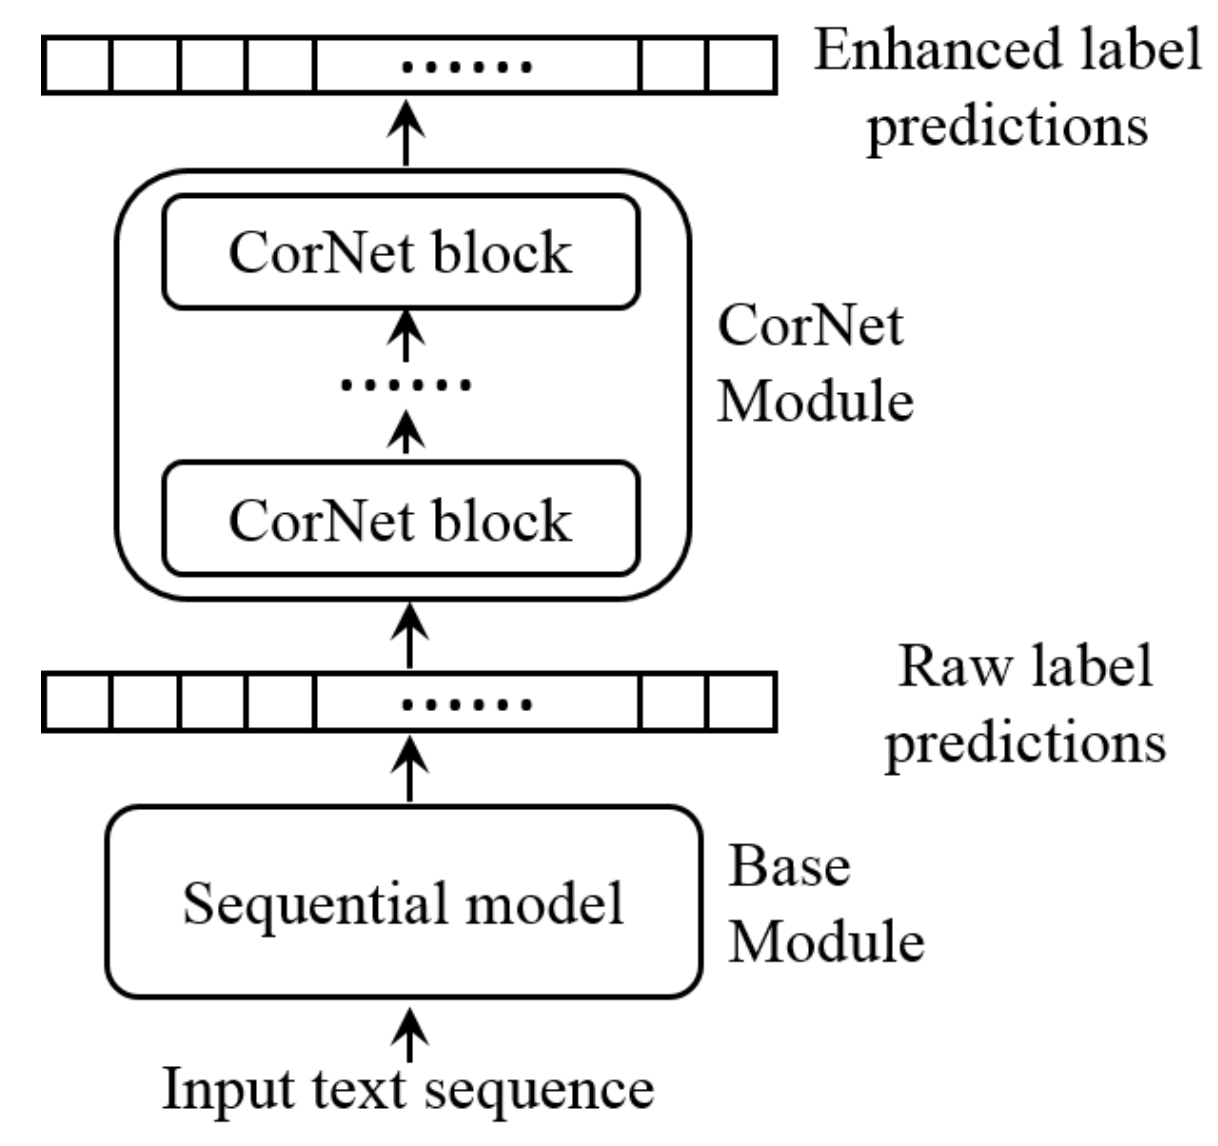
\includegraphics[width=0.7\linewidth]{images/cornet.png}
    \caption{\footnotesize{Framework of a CorNet model}}
    \label{fig:cornet}
\end{wrapfigure}

Использование CorNet в общем случае случае показано на рисунке~\ref{fig:cornet}.

То есть можно добавлять несколько CorNet слоев подряд для того чтобы выучивать более сложные корреляции между признаками. \\

\paragraph{Experiments}

Авторы проводят большое количество экспериментов с разными XMTC моделями на разных датастех, где сравнинвают качество XMTC модели с и без использования CorNet блока.

Из результов экспериментов авторы делают выводы, что использование CorNet блока: практически всегда позволяет значимо улучшить качество XMTC модели, почти не влияет на размер и время обучения.

\section*{Выводы}

\dbox{\textbf{Key Takeaways}:
\begin{enumerate}
    \item Добавление CorNet блока поверх предсказаний основной модели практически бесплатно позволяет улучшить качество модели.
    \item Добавление дополнительных CoreNet блоков позволяет дополнительно улучшить качетсво.
\end{enumerate}}

% \chapter{Taming Pretrained Transformers for eXtreme Multi-label Text Classification}

\chapter{Другие работы}

\section*{Improving Deep Learning For Airbnb Search}

Airbnb \\

\textbf{Reference:}~\cite{haldar2020improving} \\

Продолжение статьи Applying Deep Learning To Airbnb Search~\url{https://arxiv.org/pdf/1810.09591.pdf} \\

Довольно интересная статья про переход от GBDT к DL моделям в поиске Airbnb. \\

В отличии от большинства статей, в данной работе авторы большое внимание уделяют тому какие шишки они набили в процессе перехода к DL и про опыт в целом, а не просто тому какую модель они задеплоили. Не мало места они уделяют обзору того, что хорошо работает в статьях, но у них не заработало. \\

Особенно мотивирующим получился раздел RETROSPECTIVE. 


\addcontentsline{toc}{chapter}{Литература}
\putbib[refs_dl]
\end{bibunit}
